\chapter{Surface (Triangle mesh)}
\label{cap_surface}

InVesalius, generates 3D surfaces based on image segmentation. A surface is generated using the marching cubes algorithm by transforming voxels from the stacked and segmented images to polygons (triangles in this case).

The controls to configure a 3D surface are accessible on the left panel, under \textbf{3. Configure 3D surface}, \textbf{Surface properties} you have the controls to configure a 3D surface (Figure~\ref{fig:3d_surface_managment}).

\begin{figure}[!htb]
\centering
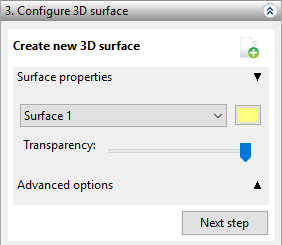
\includegraphics[scale=0.65]{surface_config_panel_en.png}
\caption{3D surface configuration.}
\label{fig:3d_surface_managment}
\end{figure}


\section{Creating 3D surfaces}

News surfaces can be created using an already segmented mask. To do so, on the left panel under \textbf{3. Configure 3D surface}, click on the button shown in Figure~\ref{fig:shortcut_new_surface}.

\begin{figure}[!htb]
\centering

\includegraphics[scale=0.18]{object_add_original}
\caption{Button to create a 3D surface.}
\label{fig:shortcut_new_surface}
\end{figure}

After clicking this button a dialog will be shown (Figure~\ref{fig:create_surface_1}). This dialog allows for the configuration of the 3D surface created, including setting the quality of the surface, filling surface holes whilst keeping the largest connected region of the surface intact.

\begin{figure}[!htb]
\centering
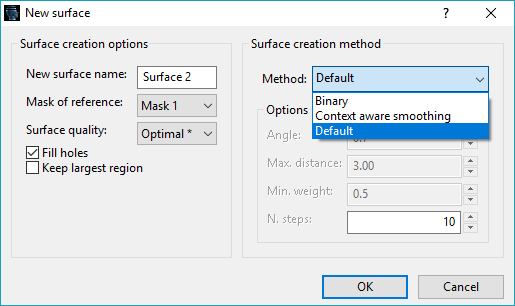
\includegraphics[scale=0.5]{surface_config_window_en.png}
\caption{3D surface creation dialog.}
\label{fig:create_surface_1}
\end{figure}

The keep largest region option may be used, for instance, to remove the tomograph supports. Figure~\ref{fig:surface_ex1} displays a surface created with \textbf{Keep largest region} and \textbf{Fill holes} activated, whereas Figure~\ref{fig:surface_ex2} displays the surface create without activating that options. Note the tomograph support and the holes.

\begin{figure}[!htb]
  \centering
  \subfloat[Frente]{\label{fig:__1}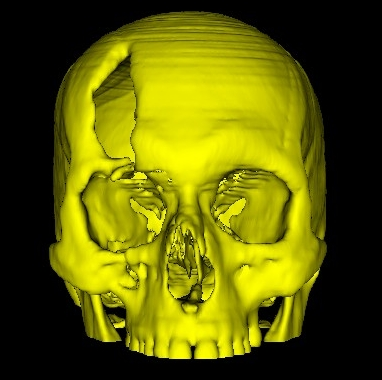
\includegraphics[width=0.338\textwidth]{surface_model_front.jpg}}
  \subfloat[Baixo]{\label{fig:__1}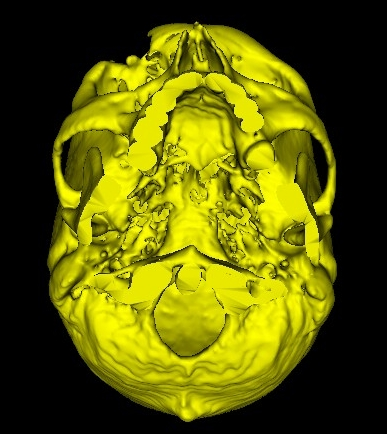
\includegraphics[width=0.3\textwidth]{surface_model_bottom.jpg}}
  \caption{Surface created with the options \textbf{Keep largest region} and \textbf{Fill holes} activated.}
  \label{fig:surface_ex1}
\end{figure}

\begin{figure}
  \centering
  \subfloat[Frente]{\label{fig:__2}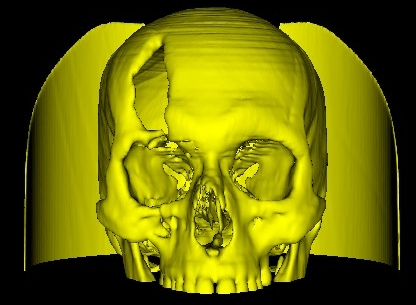
\includegraphics[width=0.371\textwidth]{surface_model_front_all_parts.jpg}}
  \subfloat[Baixo]{\label{fig:__2}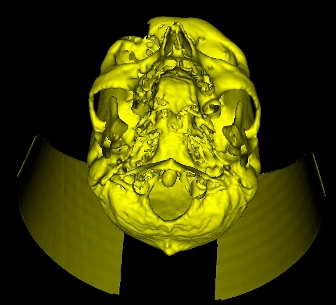
\includegraphics[width=0.3\textwidth]{surface_model_bottom_all_parts.jpg}}
  \caption{Surface created with the options \textbf{Keep largest region} and \textbf{Fill holes} deactivated.}
  \label{fig:surface_ex2}
\end{figure}

The \textbf{Surface creation method} item has the following options: \textbf{Binary}, \textbf{Context aware smoothing} and \textbf{Default}. Figure~\ref{fig:surf_method} shows an example of surface created using each of these 3 methods.

The \textbf{Binary} method takes as input the segmentation mask which is binary, where selected regions have value 1 and non-selected have value 0. As it is binary, the surface generated has a blocky aspect, mainly in high curvature areas, appearing staircases.

\textbf{Context aware smoothing} starts generating the surface using Binary, then uses another algorithm in order to smooth the surface to avoid staircase details. This method has 4 parameters presented below.

The \textbf{angle} parameter is the angle between 2 adjacent triangles. If the calculated angle is greater than the angle parameter the triangle will be considered a staircase triangle and will be smoothed. The angle parameter ranges from $0$ to $1$, where $0$ is $0^\circ$ and $1$ is $90^\circ$. The \textbf{Max distance} is the maximum distance that a non-staircase triangle may be from a staircase triangle to be considered to be smoothed. Non-staircase triangles with distance greater than Max distance also will be smoothed but the smoothing will be determined by the \textbf{Min. weight} parameter. This parameter ranges from $0$ (without smoothing) to $1$ (total smoothing). The last parameter, \textbf{N.steps}, is the number of times the smoothing algorithm will be run. The greater this parameter the smoother the surface will be.

The \textbf{Default} method is enabled only when thresholding segmentation was used without any manual modification to the mask. This method does not use the mask image, but the raw image, and generates a smoother surface.

\begin{figure}[!htb]
  \centering
  \subfloat[Binary]{\label{fig:surf_binary}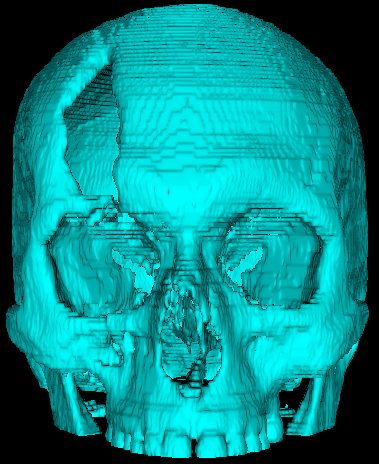
\includegraphics[width=0.33\textwidth]{binary.png}}
  \hfill
  \subfloat[Context aware]{\label{fig:surf_context}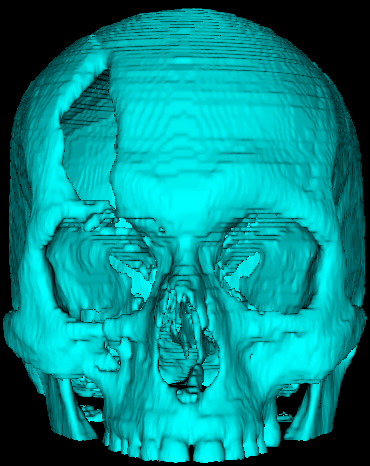
\includegraphics[width=0.32\textwidth]{context.png}}
  \hfill
  \subfloat[Default]{\label{fig:surfa_default}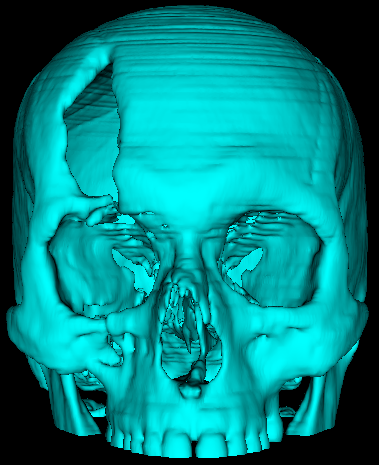
\includegraphics[width=0.332\textwidth]{default.png}}
  \caption{Surface generated by each method.}
  \label{fig:surf_method}
\end{figure}

\section{Transparency}

The Transparency function allows for the displaying of a surface transparently. To do so, select the desired surface from the list of surfaces, in the item \textbf{3. Configure 3D surface}, \textbf{Surface properties} (Figure~\ref{fig:select_surface}).

\begin{figure}[!htb]
\centering
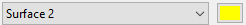
\includegraphics[scale=0.8]{surface_select_menu_en.png}
\caption{Surface selection.}
\label{fig:select_surface}
\end{figure}

Then, to set the level of surface transparency, use the sliding control shown in Figure~\ref{fig:select_transparency}; the more to the right, the more transparent the surface will be.

\begin{figure}[!htb]
\centering
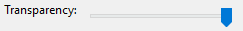
\includegraphics[scale=0.7]{surface_transparency_en.png}
\caption{Selection of surface transparency.}
\label{fig:select_transparency}
\end{figure}

Figure~\ref{fig:model_transparency} shows 2 surfaces: the external surface in green has some level of transparency which permits to see the internal surface in yellow.

\begin{figure}[!htb]
\centering
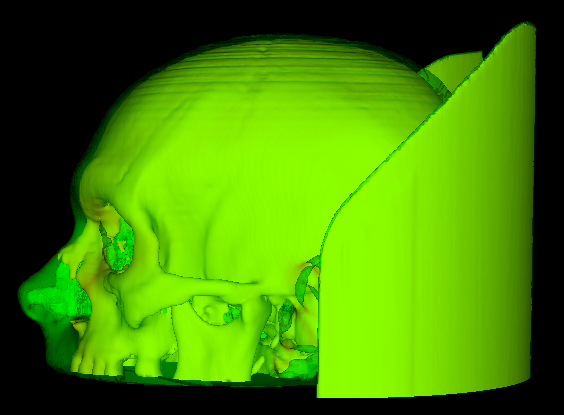
\includegraphics[scale=0.3]{transparency_2}
\caption{Surface with transparency.}
\label{fig:model_transparency}
\end{figure}

\newpage

\section{Color}

Surface colors can be altered by selecting the surface (Figure~\ref{fig:select_surface}), and clicking on the colored button on the right of the surface selection list. Figure~\ref{fig:change_surface_color} displays this button, inside item \textbf{3. Configure 3D surface}, \textbf{Surface properties}.

\begin{figure}[!htb]
\centering
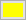
\includegraphics[scale=0.6]{surface_button_select_color_yellow.png}
\caption{Button to change surface color.}
\label{fig:change_surface_color}
\end{figure}

A dialog will be shown (Figure~\ref{fig:button_select_color}). Select the desired color and click on \textbf{OK}.

\begin{figure}[!htb]
\centering
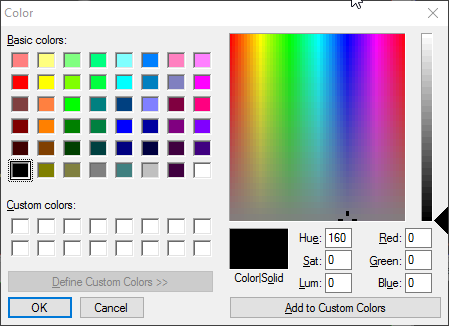
\includegraphics[scale=0.6]{surface_select_color_windows_so_en.png}
\caption{Color dialog.}
\label{fig:button_select_color}
\end{figure}

\section{Splitting disconnected surfaces}

To split disconnected surfaces, select \textbf{3. Configure 3D surface}, \textbf{Advanced options} (Figure~\ref{fig:advanced_tools}).

\begin{figure}[!htb]
\centering
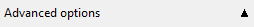
\includegraphics[scale=0.7]{surface_painel_advanced_options_en.png}
\caption{Advanced options.}
\label{fig:advanced_tools}
\end{figure}

\newpage

The advanced options panel will be displayed (Figure~\ref{fig:advanced_tools_expanded}).

\begin{figure}[!htb]
\centering
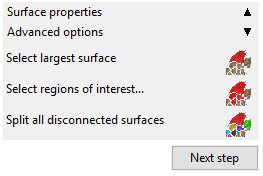
\includegraphics[scale=0.7]{surface_split_en.png}
\caption{Advanced options panel.}
\label{fig:advanced_tools_expanded}
\end{figure}

\subsection{Select largest surface}

The option \textbf{Select largest surface} selects, automatically, only surface with the greater volume. Click on the button illustrated in Figure~\ref{fig:short_connectivity_largest}. This operation creates new a surface with only the largest surface.


\begin{figure}[!htb]
\centering
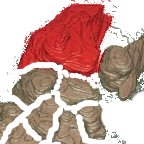
\includegraphics[scale=0.2]{connectivity_largest}
\caption{Button to split the largest disconnected surface}
\label{fig:short_connectivity_largest}
\end{figure}

As an example, the Figure~\ref{fig:extract_most_region_1} shows a surface before \textbf{Select largest surface}.

\begin{figure}[!htb]
\centering
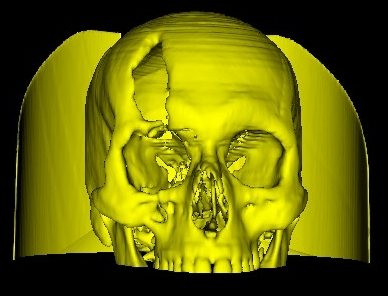
\includegraphics[scale=0.3]{surface_extract_most_region_1.jpg}
\caption{Disconnected surfaces.}
\label{fig:extract_most_region_1}
\end{figure}

Whereas the Figure~\ref{fig:extract_most_region2} shows the surface with largest disconnected region separated.

\begin{figure}[!htb]
\centering
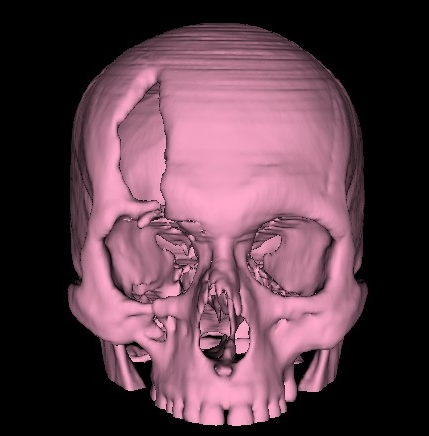
\includegraphics[scale=0.3]{surface_extract_most_region2.jpg}
\caption{Largest disconnected region separated.}
\label{fig:extract_most_region2}
\end{figure}

\newpage

\subsection{Select regions of interest}

Another selection option is Select regions of interest. To do this operation click on the button illustrated in Figure~\ref{fig:short_connectivity_manual}, then click on the desired disconnected surface regions you want to select. Next click on \textbf{Select regions of interest}. This operation will create a new surface with only the selected disconnected regions.

\begin{figure}[!htb]
\centering
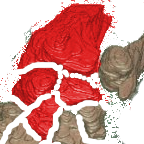
\includegraphics[scale=0.2]{connectivity_manual}
\caption{Button to select the regions of interest.}
\label{fig:short_connectivity_manual}
\end{figure}

As an example, the Figure~\ref{fig:extract_most_region3} shows the surface created after the user selects the cranium and the right part of the tomograph support.

\begin{figure}[!htb]
\centering
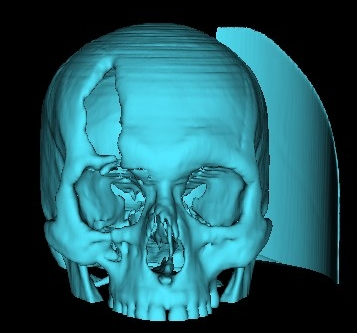
\includegraphics[scale=0.35]{surface_extract_most_region3.jpg}
\caption{Example of selected regions of interest}
\label{fig:extract_most_region3}
\end{figure}


\subsection{Split all disconnected surfaces}

Disconnected surface regions can also be split automatically. To do this, click on the button illustrated in Figure\ref{fig:connectivity_split_all}.

\begin{figure}[!htb]
\centering
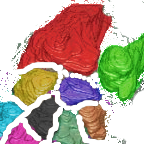
\includegraphics[scale=0.2]{connectivity_split_all}
\caption{Button to split all the disconnected regions surface.}
\label{fig:connectivity_split_all}
\end{figure}

Figure~\ref{fig:extrac_most_region_4} shows an example.

\begin{figure}[!htb]
\centering
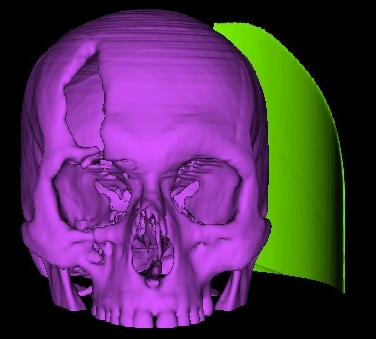
\includegraphics[scale=0.3]{surface_extract_most_region_4.jpg}
\caption{Example of split all disconnected regions surface.}
\label{fig:extrac_most_region_4}
\end{figure}

